% =====================================================================
%  Interim Progress Report (IPR) -- 10% of the module
%  Visible In-Progress (VIP) template. Expected length: 8-14 pages.
%
%  VIP rules (please read):
%   1. Commit and push after each writing session with a clear message,
%      e.g. "IPR: drafted literature review, 3 papers compared".
%   2. Your supervisor reviews your history before each meeting.
%   3. Before submitting, create a GitHub release called IPR-v1.0 with this
%      PDF attached (see 'Create your release' in the notebook).
%   4. Export the PDF and submit it on Canvas (Canvas is the official record).
%
%  REVISED after informal IPR feedback (24/11/2026): the project was
%  re-scoped to hand-crafted numerical features + Decision Tree and SVM
%  (code in tb_ml/).
%  Search for \todo to find the places you still need to fill in.
% =====================================================================
\documentclass[11pt,a4paper]{article}
\usepackage{vip}

% ---------- (vip.sty already loads graphicx, booktabs, tabularx, listings, xcolor) ----
\newcommand{\todo}[1]{\textcolor{red}{\textbf{[TODO: #1]}}}
\lstset{language=Python}

% ---------- EDIT YOUR DETAILS ----------------------------------------
\projecttitle{Detecting Tuberculosis in Chest X-rays with Numerical Image Features and Classical Machine Learning: A Within- and Cross-Dataset Study on the Montgomery and Shenzhen Sets}
\studentname{Izuchukwu Agballah}
\studentnumber{12345678} % TODO: the notebook gives 24136661 -- check which is correct
\supervisor{Muhammad Yaqoob}
\modulecode{7COM1039}
\moduletitle{MSc Project}
\reporttype{Interim Progress Report (IPR)}
\gitrepo{https://github.com/Izuchukwu-A/msc-project-agballah.git}
\gitrelease{IPR-v1.0}   % the release you create before submitting


\begin{document}
\makecoverpage
\makecontents

\section{Background Research and Literature Review}
\subsection{Goals and Objectives}
Tuberculosis (TB) remains one of the most common fatal infections in the world, and for most patients the first test is a chest X-ray. The countries with the heaviest TB burden tend to have the fewest radiologists, so an automated reader that flags likely TB cases could help. The US National Library of Medicine released two public TB chest X-ray datasets: the Montgomery County set (138 images, 58 TB and 80 normal) and the Shenzhen set (662 images, 336 TB and 326 normal) \citep{jaeger2014}. Because they come from two hospitals in two countries, they also allow a simple test of whether a model trained in one hospital still works in another.

\noindent\textbf{Aim.} To find out how well TB can be detected in chest X-rays using a small set of numerical features extracted from each image (intensity, texture and edge features) and two classical machine learning models, a Decision Tree and a Support Vector Machine (SVM), and to test whether a model trained on one hospital's images works on the other's.

\noindent\textbf{Objectives.}
\begin{enumerate}\itemsep2pt
  \item Review the literature on extracting numerical features from chest X-rays and on the machine learning models used with them for TB detection.
  \item Download and inspect both datasets and check them for problems such as duplicate images.
  \item Extract 13 numerical features from every image: six intensity, five texture (GLCM) and two edge features.
  \item Train and evaluate a Decision Tree and an SVM on each dataset with repeated stratified five-fold cross-validation.
  \item Find out which group of features (intensity, texture or edges) carries the most useful information.
  \item Train on one dataset and test on the other, in both directions, and measure the drop in performance.
  \item Compare the results with published work on the same datasets.
\end{enumerate}

\noindent\textbf{Scope.} Binary TB-versus-normal classification of frontal chest X-rays from the two NLM datasets, using hand-crafted features and two classical models. Deep learning, lung segmentation, other datasets and any clinical deployment are outside the scope.

\subsection{Research Questions}
\begin{enumerate}\itemsep2pt
  \item How accurately can a Decision Tree and an SVM detect TB from 13 numerical image features, within each dataset?
  \item Which of the two models performs better, and why?
  \item Which feature group (intensity, texture or edges) is most useful for detecting TB?
  \item How much does performance drop when a model trained on one hospital's images is tested on the other's?
\end{enumerate}

\subsection{Background Research}
\noindent\textbf{Numerical features from chest X-rays. }Before deep learning, computer-aided TB screening described each X-ray with a set of hand-crafted numerical features and passed them to a standard classifier. \citet{jaeger2014tmi} segmented the lungs and computed intensity, edge, shape and texture descriptors inside them, then classified the images with an SVM. They reported an area under the ROC curve (AUC) of 0.87 on Montgomery and 0.90 on Shenzhen, and this is the main published baseline for the method used here. Texture features are commonly computed from the grey-level co-occurrence matrix (GLCM) of \citet{haralick1973}, which counts how often pairs of grey levels occur next to each other. TB lesions such as consolidation, cavities and nodules change the local texture of the lung, which these features can capture.

\noindent\textbf{Machine learning models used with these features. }The SVM \citep{cortes1995} is the classifier most often used with hand-crafted chest X-ray features, including by \citet{jaeger2014tmi}. Tree-based models also appear: \citet{santosh2018} combined shape, edge and texture features describing the symmetry of the two lungs, and classified them with a vote between a Bayesian network, a multilayer perceptron and a random forest (an ensemble of decision trees). The Decision Tree \citep{breiman1984} was chosen as the second model because it is the building block of the random forest and because its decisions can be read directly from the tree.

\noindent\textbf{Deep learning and cross-hospital performance. }More recent work uses convolutional neural networks, which learn features directly from the pixels. \citet{pasa2019} showed that a small network performs well on these datasets. Deep models are harder to interpret, though, and there is evidence that they can learn which hospital an image came from rather than the disease: \citet{zech2018} found that a pneumonia model performed worse at hospitals it had not been trained on. \citet{hansun2024} found the same kind of drop on the Montgomery and Shenzhen sets. This project uses simple, interpretable models instead and runs the same cross-hospital test on them. Table~\ref{tab:lit} summarises the sources.

\begin{table}[htbp]
  \centering
  \caption{Core sources: approach, features, model and relevance to this project.}
  \label{tab:lit}
  \footnotesize
  \begin{tabularx}{\linewidth}{>{\raggedright\arraybackslash}p{0.17\linewidth} >{\raggedright\arraybackslash}p{0.2\linewidth} >{\raggedright\arraybackslash}p{0.17\linewidth} X}
    \toprule
    \textbf{Study} & \textbf{Features} & \textbf{Model} & \textbf{Relevance} \\
    \midrule
    \citet{jaeger2014} & Dataset release & -- & Defines the two datasets \\
    \citet{jaeger2014tmi} & Intensity, edge, shape, texture inside segmented lungs & SVM & Main published baseline: AUC 0.87 (MC), 0.90 (SZ) \\
    \citet{haralick1973} & GLCM texture & -- & Source of the texture features \\
    \citet{santosh2018} & Shape, edge, texture; lung symmetry & Bayes net + MLP + random forest (vote) & Tree-based model with hand-crafted features \\
    \citet{pasa2019} & Learned (CNN) & Compact CNN & Deep learning comparison \\
    \citet{zech2018} & Learned (CNN) & CNN, pneumonia & Performance drops at an unseen hospital \\
    \citet{hansun2024} & Learned (CNN) & EfficientNet ensemble & Cross-dataset drop on MC and SZ \\
    \bottomrule
  \end{tabularx}
\end{table}

\todo{Add the papers you read each week (two per week, from the Excel sheet) to this section and to Table~\ref{tab:lit}. Read every source in full before citing it.}

\section{Summary of Progress to Date}
\subsection{Dataset Preparation and Exploratory Analysis}
Both sets were downloaded from the NLM repository with a script (\texttt{step0\_download\_data.py}), and the counts were checked against the published figures (Table~\ref{tab:data}). The label is the last digit of each filename (\texttt{\_0} normal, \texttt{\_1} TB). All 800 images were checked for duplicates: no two files are byte-identical, and comparing small thumbnails of every pair found no near-duplicates (the most similar pair had a correlation of 0.966). The same X-ray therefore cannot appear in both a training fold and a test fold.

\begin{table}[htbp]
  \centering
  \caption{The two NLM datasets as published and verified on download.}
  \label{tab:data}
  \footnotesize
  \begin{tabularx}{\linewidth}{l X X}
    \toprule
    \textbf{} & \textbf{Montgomery County (USA)} & \textbf{Shenzhen (China)} \\
    \midrule
    Setting & County TB screening programme & Hospital out-patient clinics \\
    Images & 138 & 662 \\
    TB / normal & 58 / 80 & 336 / 326 \\
    TB prevalence & 42\% & 51\% \\
    Resolution & About 4020 $\times$ 4892 & About 3000 $\times$ 3000, varies \\
    File format & 8-bit greyscale PNG & 8-bit PNG (palette or RGB), converted to greyscale \\
    \bottomrule
  \end{tabularx}
\end{table}

Every image is converted to greyscale and resized to 256 $\times$ 256 pixels so that the features are comparable. Figure~\ref{fig:samples} shows that the two hospitals' images look different: Montgomery images have wide black borders and burned-in text labels (``PA ERECT''), while Shenzhen images are framed more tightly. These differences have nothing to do with TB, but whole-image features will still pick them up. This matters for the cross-dataset test (Section~\ref{sec:results}).

\begin{figure}[htbp]
  \centering
  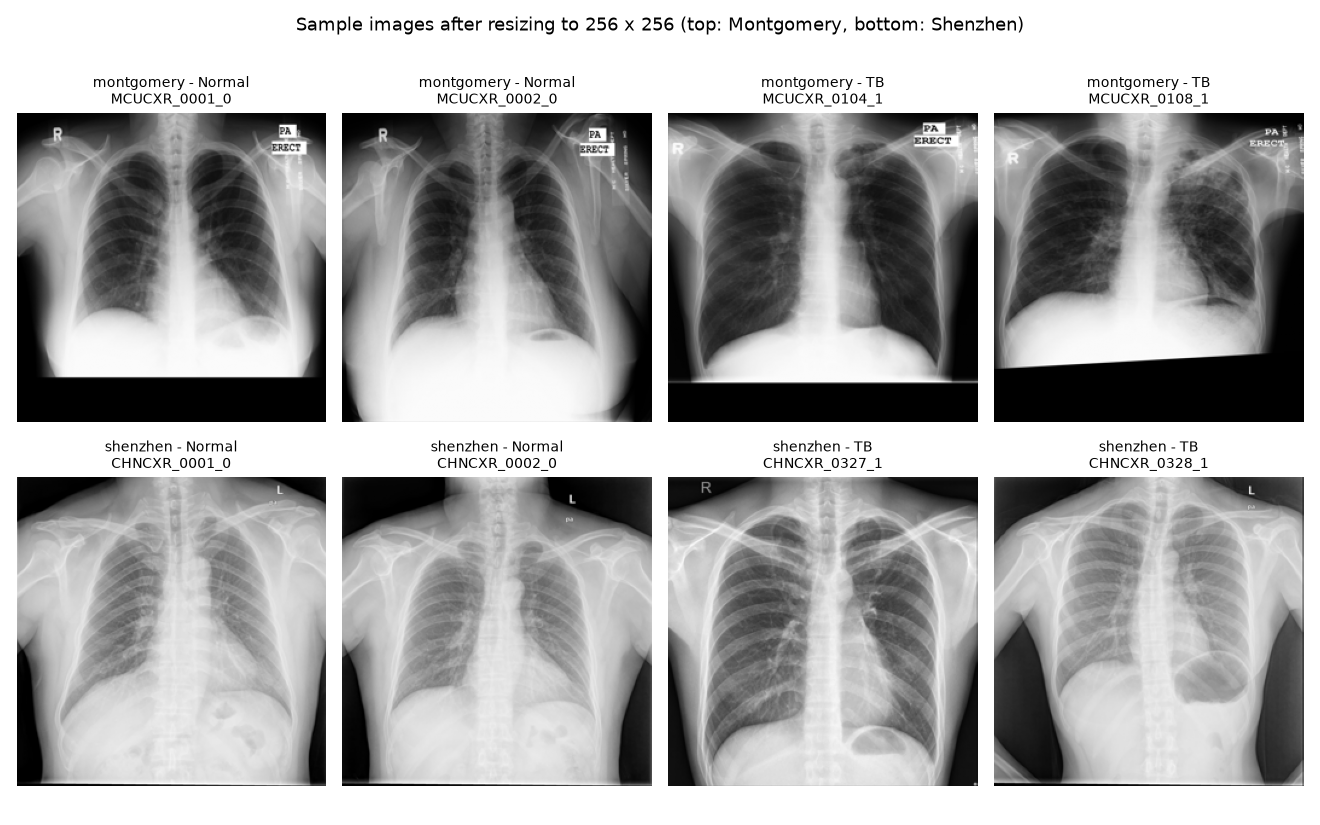
\includegraphics[width=0.85\linewidth]{fig_samples.png}
  \caption{Two normal and two TB images from each dataset after resizing. Montgomery (top) has black borders and text labels that Shenzhen (bottom) does not.}
  \label{fig:samples}
\end{figure}

\subsection{Feature Extraction}
Thirteen numerical features are computed from each image in three groups (Table~\ref{tab:features}). The texture features come from the GLCM: the image is reduced to 32 grey levels, pairs of neighbouring pixels one pixel apart are counted in four directions (0$^\circ$, 45$^\circ$, 90$^\circ$, 135$^\circ$), and each Haralick property is averaged over the four directions \citep{haralick1973}. Figure~\ref{fig:boxplots} compares the distribution of each feature for normal and TB images.

\begin{table}[htbp]
  \centering
  \caption{The 13 features extracted from each image.}
  \label{tab:features}
  \footnotesize
  \begin{tabularx}{\linewidth}{l l X}
    \toprule
    \textbf{Group} & \textbf{Features} & \textbf{What they measure} \\
    \midrule
    Intensity (6) & mean, median, std, skewness, kurtosis, entropy & Overall brightness, spread and shape of the grey-level histogram \\
    Texture (5) & GLCM contrast, dissimilarity, homogeneity, energy, correlation & How neighbouring pixels relate: smooth versus patchy regions \\
    Edges (2) & mean and std of Sobel gradient magnitude & How many sharp brightness changes the image contains \\
    \bottomrule
  \end{tabularx}
\end{table}

\begin{figure}[htbp]
  \centering
  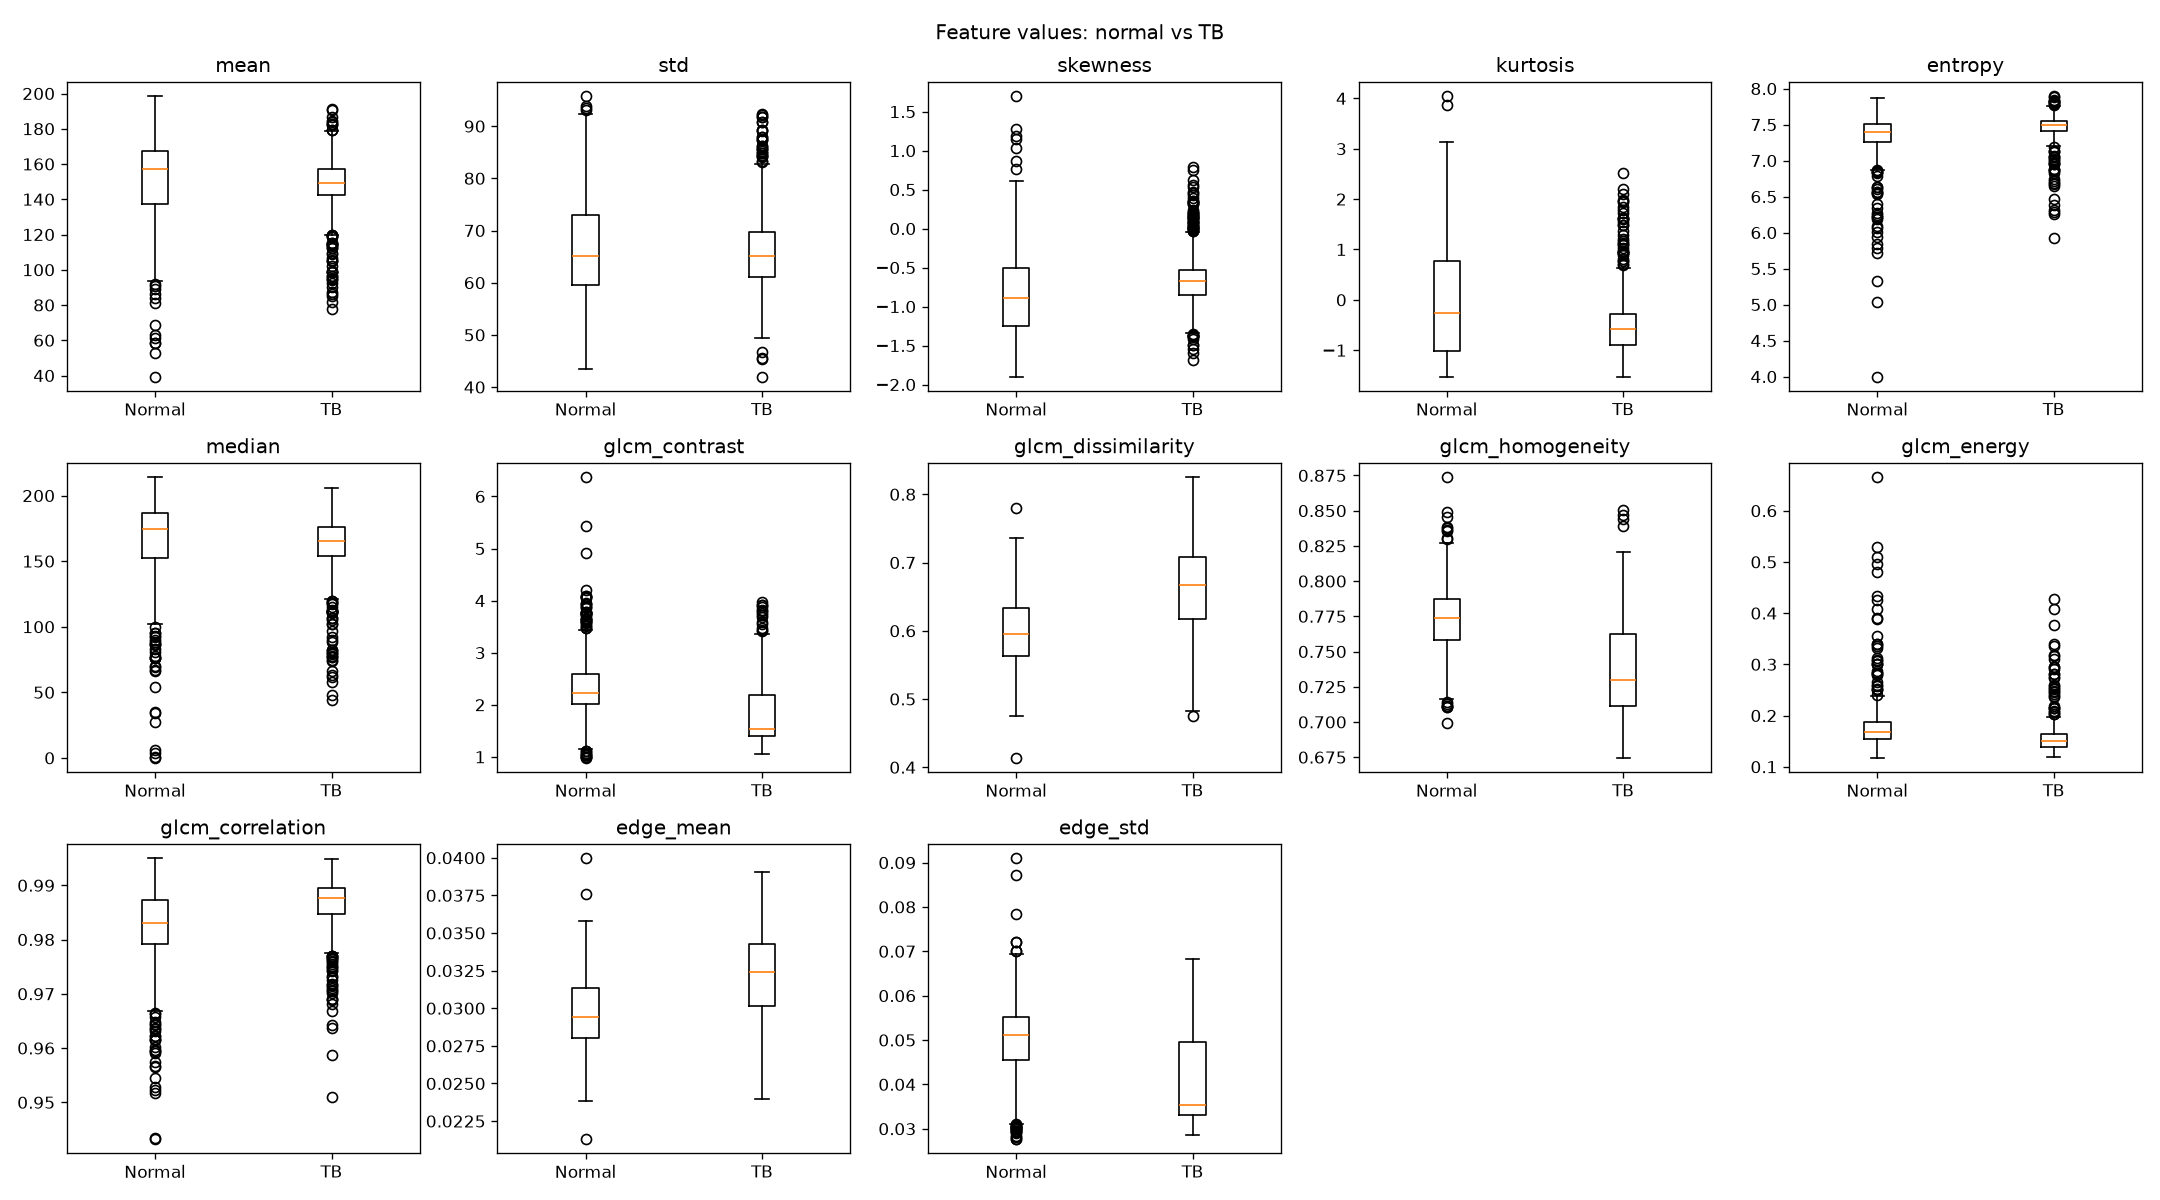
\includegraphics[width=0.95\linewidth]{fig_boxplots.png}
  \caption{Distribution of each feature for normal and TB images (both datasets).}
  \label{fig:boxplots}
\end{figure}

\subsection{Model Development and Tools}
\noindent\textbf{Decision Tree. }A decision tree learns a sequence of yes/no questions about single features (for example ``is GLCM contrast above 12.3?''), choosing at each step the question that best separates the two classes, measured by Gini impurity \citep{breiman1984}. The maximum depth (2--6) and the minimum number of images per leaf (1, 5 or 10) are tuned so that the tree does not memorise the training images.

\noindent\textbf{SVM. }An SVM with a radial basis function (RBF) kernel finds the boundary between the classes that leaves the widest margin to the nearest training images \citep{cortes1995}. The penalty $C$ (0.1--100) and the kernel width $\gamma$ are tuned. Because the SVM works with distances between images, the features are first standardised to mean 0 and standard deviation 1.

\noindent\textbf{Evaluation. }Each dataset is evaluated with repeated stratified five-fold cross-validation: the images are split into five parts with the same TB/normal ratio, each part is used once as the test set, and the whole procedure is repeated five times with different shuffles. This gives 25 test results, which are reported as mean $\pm$ standard deviation. Inside each training part, the hyperparameters are chosen by a further five-fold cross-validation, so the test images are never used to choose settings \citep{varma2006}. A single 80/20 split was tried first and rejected: on Montgomery it left only 28 test images, so one image changed the accuracy by about four percentage points. The metrics are accuracy, sensitivity, specificity, precision, F1 and AUC, with TB as the positive class.

\noindent\textbf{Tools. }Python 3.14 with NumPy, pandas, SciPy and Pillow for data handling, scikit-image for the GLCM and Sobel features, scikit-learn for the models, cross-validation and metrics, and Matplotlib for the figures. Everything runs on a laptop CPU in a few minutes. The code is a set of four numbered scripts in the \texttt{tb\_ml} folder of the Git repository.

\subsection{Results}\label{sec:results}
\noindent\textbf{Within each dataset (RQ1, RQ2). }Table~\ref{tab:within} shows the results. On Shenzhen both models work reasonably well, and the SVM reaches an AUC of 0.860, within about 0.04 of the 0.90 reported by \citet{jaeger2014tmi}. Montgomery is much harder: the best AUC is 0.655, and the results vary a lot between folds. The SVM is better than the Decision Tree on both datasets. Figure~\ref{fig:roc} shows the ROC curves.

\begin{table}[htbp]
  \centering
  \caption{Within-dataset results: mean $\pm$ standard deviation over 25 test folds (5-fold CV repeated 5 times).}
  \label{tab:within}
  \footnotesize
  \begin{tabularx}{\linewidth}{l l X X X X}
    \toprule
    \textbf{Dataset} & \textbf{Model} & \textbf{AUC} & \textbf{Accuracy} & \textbf{Sensitivity} & \textbf{Specificity} \\
    \midrule
    Montgomery & Decision Tree & 0.548 $\pm$ 0.080 & 0.561 $\pm$ 0.068 & 0.398 $\pm$ 0.210 & 0.680 $\pm$ 0.154 \\
    Montgomery & SVM & 0.655 $\pm$ 0.076 & 0.616 $\pm$ 0.062 & 0.411 $\pm$ 0.205 & 0.765 $\pm$ 0.147 \\
    Shenzhen & Decision Tree & 0.827 $\pm$ 0.033 & 0.772 $\pm$ 0.036 & 0.734 $\pm$ 0.063 & 0.812 $\pm$ 0.070 \\
    Shenzhen & SVM & 0.860 $\pm$ 0.038 & 0.784 $\pm$ 0.034 & 0.733 $\pm$ 0.050 & 0.837 $\pm$ 0.060 \\
    \bottomrule
  \end{tabularx}
\end{table}

\begin{figure}[htbp]
  \centering
  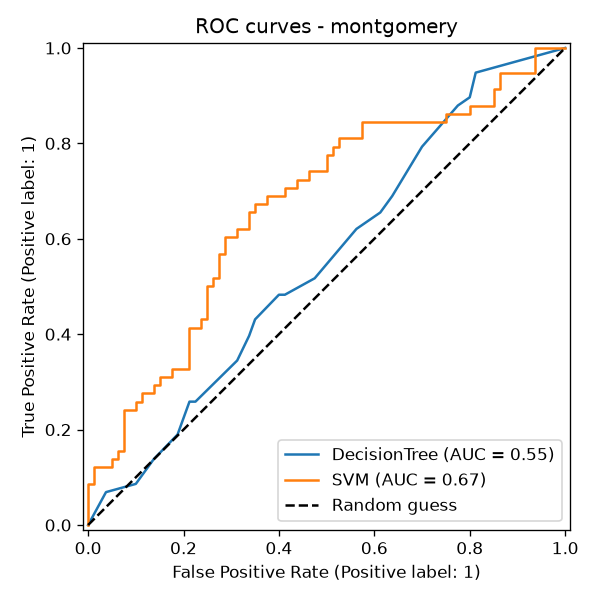
\includegraphics[width=0.42\linewidth]{fig_roc_montgomery.png}\hfill
  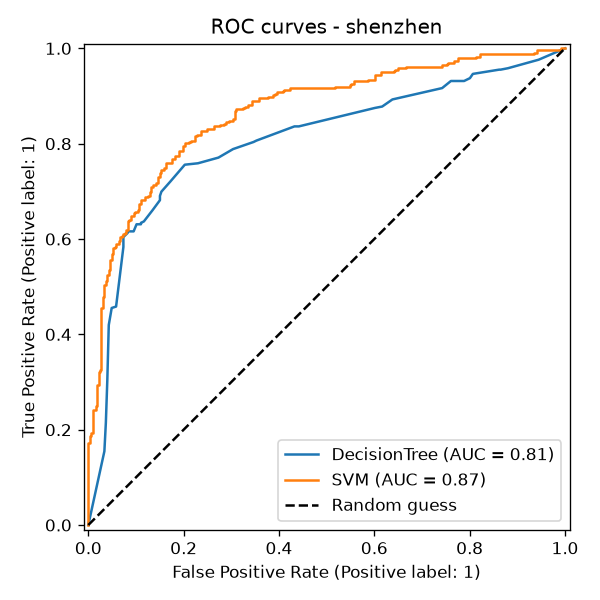
\includegraphics[width=0.42\linewidth]{fig_roc_shenzhen.png}
  \caption{ROC curves for Montgomery (left) and Shenzhen (right), first repeat of the cross-validation (every image tested once).}
  \label{fig:roc}
\end{figure}

\noindent\textbf{Which features matter (RQ3). }Table~\ref{tab:groups} and Figure~\ref{fig:groups} show the AUC when each model uses only one feature group. On Shenzhen, the five texture features alone reach 0.845 with the SVM, almost as good as all 13 features (0.860), and the two edge features alone reach 0.814. Intensity features are the weakest group on Shenzhen. On Montgomery no group clearly stands out, and all results are close to each other given the spread across folds.

\begin{table}[htbp]
  \centering
  \caption{AUC per feature group (mean $\pm$ std over 25 folds).}
  \label{tab:groups}
  \footnotesize
  \begin{tabularx}{\linewidth}{l l X X X X}
    \toprule
    \textbf{Dataset} & \textbf{Model} & \textbf{Intensity (6)} & \textbf{Texture (5)} & \textbf{Edges (2)} & \textbf{All (13)} \\
    \midrule
    Montgomery & Decision Tree & 0.547 $\pm$ 0.088 & 0.513 $\pm$ 0.087 & 0.583 $\pm$ 0.099 & 0.548 $\pm$ 0.080 \\
    Montgomery & SVM & 0.657 $\pm$ 0.096 & 0.602 $\pm$ 0.075 & 0.610 $\pm$ 0.085 & 0.655 $\pm$ 0.076 \\
    Shenzhen & Decision Tree & 0.723 $\pm$ 0.045 & 0.819 $\pm$ 0.038 & 0.811 $\pm$ 0.041 & 0.827 $\pm$ 0.033 \\
    Shenzhen & SVM & 0.806 $\pm$ 0.036 & 0.845 $\pm$ 0.037 & 0.814 $\pm$ 0.033 & 0.860 $\pm$ 0.038 \\
    \bottomrule
  \end{tabularx}
\end{table}

\begin{figure}[htbp]
  \centering
  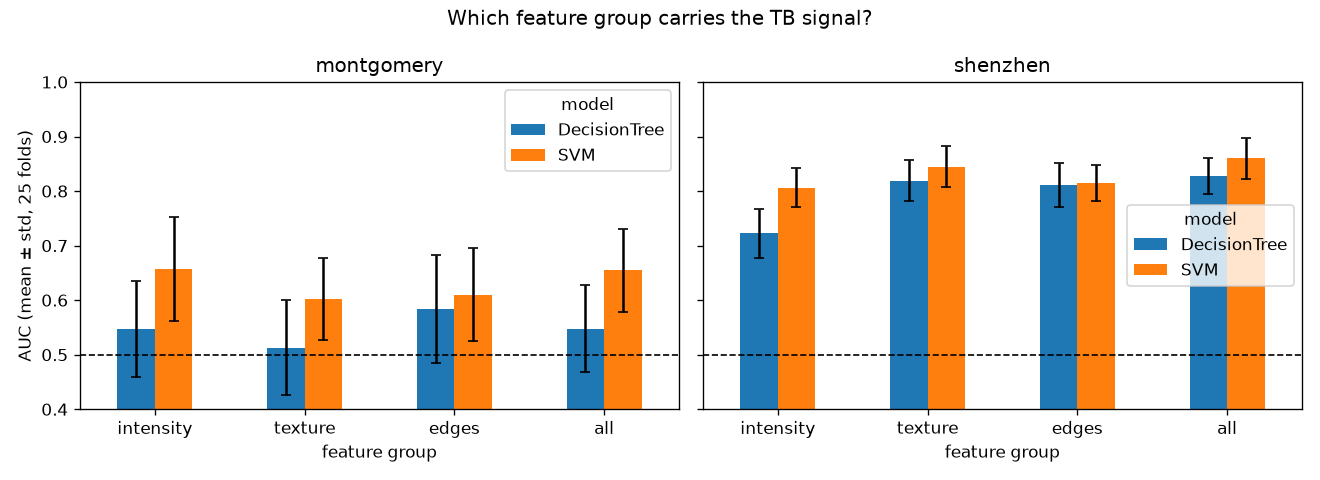
\includegraphics[width=0.9\linewidth]{fig_groups.png}
  \caption{AUC per feature group. Error bars show the standard deviation over 25 folds; the dashed line is chance (0.5).}
  \label{fig:groups}
\end{figure}

\noindent\textbf{Cross-dataset (RQ4). }Table~\ref{tab:cross} shows what happens when a model is trained on all images from one hospital and tested on all images from the other. In three of the four cases performance falls to around chance, and the model predicts ``normal'' for almost every image: trained on Shenzhen and tested on Montgomery, the SVM finds none of the 58 TB cases. The exception is the SVM trained on Montgomery and tested on Shenzhen, which keeps an AUC of 0.825.

\begin{table}[htbp]
  \centering
  \caption{Cross-dataset results: train on all of one set, test once on all of the other.}
  \label{tab:cross}
  \footnotesize
  \begin{tabularx}{\linewidth}{X l c c c c}
    \toprule
    \textbf{Train $\rightarrow$ Test} & \textbf{Model} & \textbf{AUC} & \textbf{Accuracy} & \textbf{Sensitivity} & \textbf{Specificity} \\
    \midrule
    Shenzhen $\rightarrow$ Montgomery & Decision Tree & 0.535 & 0.580 & 0.052 & 0.962 \\
    Shenzhen $\rightarrow$ Montgomery & SVM & 0.468 & 0.580 & 0.000 & 1.000 \\
    Montgomery $\rightarrow$ Shenzhen & Decision Tree & 0.557 & 0.492 & 0.000 & 1.000 \\
    Montgomery $\rightarrow$ Shenzhen & SVM & 0.825 & 0.731 & 0.565 & 0.902 \\
    \bottomrule
  \end{tabularx}
\end{table}

\noindent\textbf{Comparison with published work. }\citet{jaeger2014tmi} reported AUCs of 0.87 (Montgomery) and 0.90 (Shenzhen). The gap is small on Shenzhen and large on Montgomery, and three differences are likely to explain it. First, they computed their features inside the segmented lungs, while this project uses the whole image, including borders and text labels. Second, they used a much larger feature set. Third, Montgomery has only 138 images, so each training fold has about 110, which is very few for learning a reliable boundary. \todo{Check the exact evaluation protocol in \citet{jaeger2014tmi} and describe it here.}

\subsection{Problems Encountered}
\noindent\textbf{Scope. }The first version of the project used deep learning (CNNs), a U-Net for lung segmentation, intensity corrections and advanced statistical tests. After the informal IPR feedback, the project was re-scoped to methods that can be fully explained and justified from the literature: hand-crafted features with a Decision Tree and an SVM. The code was rewritten from scratch as four short scripts.

\noindent\textbf{Unreliable single split. }A single 80/20 split gave a Montgomery test set of only 28 images, and the Decision Tree's AUC on it (0.667) turned out to be much higher than its average over 25 folds (0.548). Repeated cross-validation was adopted to give a reliable estimate with a measure of spread.

\noindent\textbf{Software. }scikit-learn 1.9 deprecated probability outputs from the SVM, so the SVM's decision function (its signed distance from the boundary) is used as the score for the ROC curve and AUC instead.

\noindent\textbf{Hospital differences. }The cross-dataset collapse (Table~\ref{tab:cross}) suggests that whole-image features capture differences between the two hospitals' images, such as borders and exposure, as well as disease. This is recorded as a limitation and will be discussed in the final report.

\subsection{Evidence of Work Completed}
\begin{itemize}\itemsep2pt
  \item Literature review of feature extraction and classical models for TB detection (Table~\ref{tab:lit}).
  \item Both datasets downloaded, counts verified and checked for duplicate images.
  \item 13 numerical features extracted from all 800 images.
  \item Decision Tree and SVM evaluated with repeated stratified five-fold cross-validation on each dataset.
  \item Feature-group experiment and cross-dataset experiment in both directions.
  \item All code, results and figures in the Git repository (\texttt{tb\_ml/}), reproducible with a fixed seed (42).
\end{itemize}

\section{Ethical, Legal, Professional and Social Issues}
This project uses two publicly available chest X-ray datasets released by the US National Library of Medicine, so it involves no new data collection and no contact with human participants. The images were de-identified by the dataset creators before release \citep{jaeger2014}. The ethical risk is therefore judged minimal, and the supervisor will be consulted on whether the module's ethics self-declaration is needed for secondary use of open data.

Legally, the datasets are distributed publicly for research use. The project complies with the providers' terms by citing the dataset paper and by not redistributing the images: the image folder is excluded from the Git repository. Because the data is anonymised, it does not fall under the UK GDPR as personal data.

Professionally, the work follows the BCS Code of Conduct on honesty and competence: all results are reported, including weak and negative ones such as the cross-dataset collapse, and the code is shared so the results can be reproduced. Socially, a TB screening tool that fails silently at a new hospital would delay diagnosis for the people it is meant to help. The project is therefore framed as a research evaluation, not a clinical tool.

\section{Project Plan}
The project was re-planned after the informal IPR feedback of 24/11/2026. Table~\ref{tab:phases} shows the phases and Table~\ref{tab:remaining} the remaining tasks. \todo{Check every date against the official FPR deadline. The earlier plan wrongly set the write-up for 16/02/2027.}

\begin{table}[htbp]
  \centering
  \caption{Project phases and status.}
  \label{tab:phases}
  \small
  \begin{tabularx}{\linewidth}{l l X l}
    \toprule
    \textbf{Phase} & \textbf{Weeks} & \textbf{Key tasks} & \textbf{Status} \\
    \midrule
    Phase 1 & 1--2 & Literature review and proposal & Complete \\
    Phase 2 & 3--4 & Dataset download, verification and inspection & Complete \\
    Phase 3 & 5--9 & First pipeline (deep learning), replaced after IPR feedback & Superseded \\
    Phase 4 & 9--10 & Feature extraction, Decision Tree and SVM, cross-validation & Complete \\
    Phase 5 & 10 & Feature-group and cross-dataset experiments & Complete \\
    Phase 6 & 10--11 & Further reading (two papers per week), discussion and limitations & In progress \\
    Phase 7 & 11--12 & FPR write-up, GitHub release and demo preparation & Planned \\
    \bottomrule
  \end{tabularx}
\end{table}

\begin{table}[htbp]
  \centering
  \caption{Remaining tasks.}
  \label{tab:remaining}
  \small
  \begin{tabularx}{\linewidth}{X X l}
    \toprule
    \textbf{Task} & \textbf{Deliverable} & \textbf{Target date} \\
    \midrule
    Read two papers per week on feature extraction and models & Excel sheet and literature review & Weekly \\
    Compare with \citet{jaeger2014tmi} in detail & Discussion section & \todo{date} \\
    Discussion of limitations (whole-image features, small dataset) & Discussion section & \todo{date} \\
    FPR write-up & Full FPR draft to supervisor & \todo{date} \\
    GitHub release and demo & Tagged release and demonstration & \todo{FPR deadline} \\
    \bottomrule
  \end{tabularx}
\end{table}

\begin{table}[htbp]
  \centering
  \caption{Risk register.}
  \label{tab:risk}
  \small
  \begin{tabularx}{\linewidth}{X l X}
    \toprule
    \textbf{Risk} & \textbf{Likelihood / Impact} & \textbf{Mitigation} \\
    \midrule
    Montgomery's 138 images give unreliable results & High / Medium & Repeated cross-validation; spread reported with every result \\
    Hyperparameters tuned on test data (leakage) & Low / High & Settings chosen inside each training fold only \\
    Unable to explain a method in the viva & Medium / High & Only simple methods used; each one studied and documented in the code \\
    Write-up compresses at the end & Medium / High & Sections drafted as each experiment finishes \\
    \bottomrule
  \end{tabularx}
\end{table}

\section{Level of the Project}
The project is at Master's level in three ways. First, it works with real medical images from two hospitals and tests the method under a realistic condition, a change of hospital, rather than reporting within-dataset accuracy only. Second, the evaluation is careful: hyperparameters are chosen inside each training fold only, results are averaged over 25 test folds with their spread reported, and the results are compared critically with published work. Third, the feature-group and cross-dataset experiments go beyond reporting a single accuracy figure and ask why the models succeed or fail. Every method used can be explained from first principles, and the code is short enough to be read in full.

% =====================================================================
\clearpage\phantomsection
\addcontentsline{toc}{section}{References}
\bibliographystyle{agsm}
\bibliography{refs}

\begin{appendices}
\section{Additional Results}\label{app:results}
Figure~\ref{fig:importance} shows which features a Decision Tree trained on the whole Shenzhen set relied on, and Figure~\ref{fig:confusion} shows the confusion matrices for Shenzhen.

\begin{figure}[htbp]
  \centering
  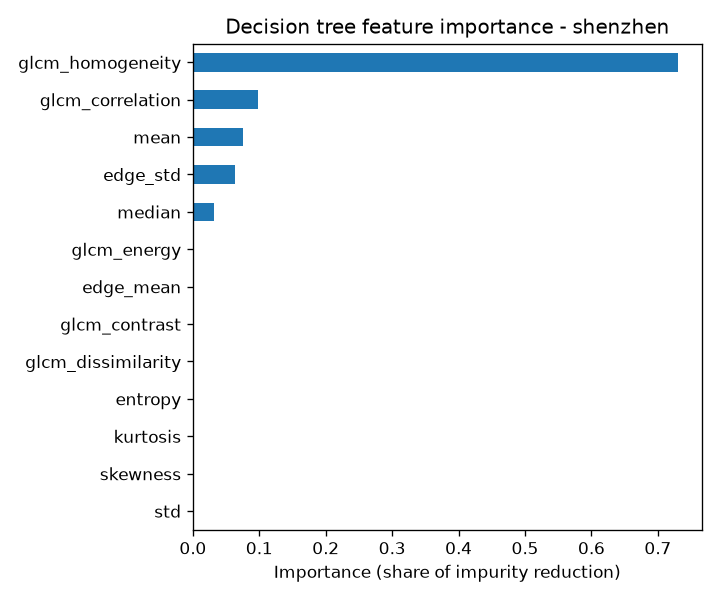
\includegraphics[width=0.55\linewidth]{fig_tree_importance.png}
  \caption{Decision Tree feature importance on Shenzhen (share of the total impurity reduction).}
  \label{fig:importance}
\end{figure}

\begin{figure}[htbp]
  \centering
  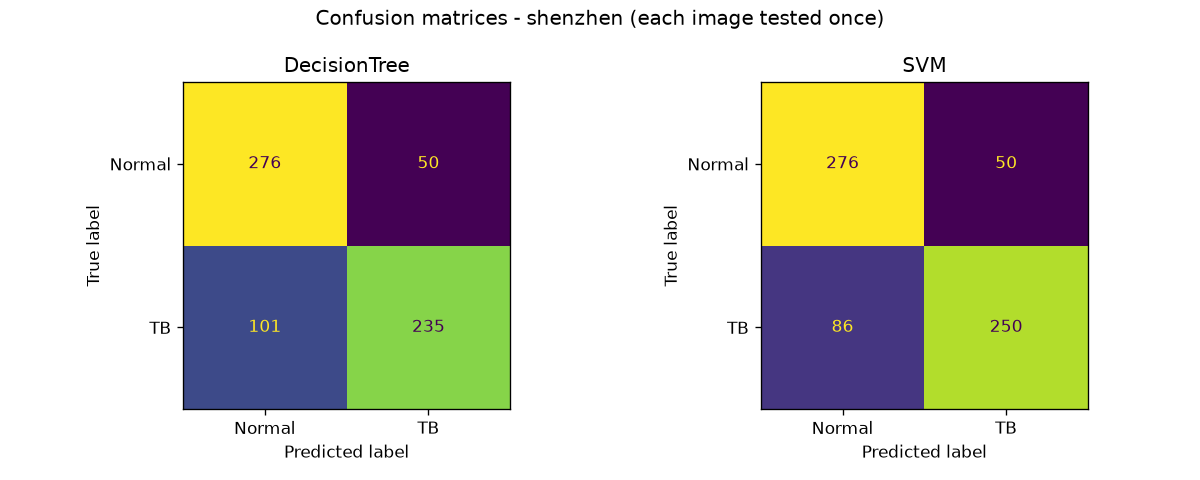
\includegraphics[width=0.8\linewidth]{fig_confusion_shenzhen.png}
  \caption{Confusion matrices on Shenzhen, first repeat of the cross-validation (every image tested once).}
  \label{fig:confusion}
\end{figure}

\section{Key Code Listings}
\noindent \texttt{tb\_ml/features.py} -- GLCM texture features for one image.
\begin{lstlisting}
def texture_features(img):
    reduced = (img // (256 // GLCM_LEVELS)).astype(np.uint8)  # 0..31
    glcm = graycomatrix(reduced, distances=[1],
                        angles=[0, np.pi/4, np.pi/2, 3*np.pi/4],
                        levels=GLCM_LEVELS, symmetric=True, normed=True)
    feats = {}
    for prop in ["contrast", "dissimilarity", "homogeneity", "energy", "correlation"]:
        feats[f"glcm_{prop}"] = graycoprops(glcm, prop).mean()
    return feats
\end{lstlisting}

\noindent \texttt{tb\_ml/models.py} -- the two models and the settings tried for each.
\begin{lstlisting}
def make_models():
    tree = DecisionTreeClassifier(random_state=SEED)
    tree_grid = {"max_depth": [2, 3, 4, 5, 6], "min_samples_leaf": [1, 5, 10]}
    svm = Pipeline([("scale", StandardScaler()),
                    ("svm", SVC(kernel="rbf", random_state=SEED))])
    svm_grid = {"svm__C": [0.1, 1, 10, 100], "svm__gamma": ["scale", 0.01, 0.1]}
    return {"DecisionTree": (tree, tree_grid), "SVM": (svm, svm_grid)}
\end{lstlisting}

\noindent \texttt{tb\_ml/models.py} -- repeated stratified five-fold cross-validation; settings are chosen inside each training fold.
\begin{lstlisting}
def repeated_cv(model, grid, X, y):
    cv = RepeatedStratifiedKFold(n_splits=5, n_repeats=5, random_state=SEED)
    rows = []
    for i, (train_idx, test_idx) in enumerate(cv.split(X, y)):
        best, params, _ = tune_and_fit(model, grid, X[train_idx], y[train_idx])
        metrics, scores = evaluate(best, X[test_idx], y[test_idx])
        rows.append({"repeat": i // 5, "fold": i % 5, **metrics})
    return pd.DataFrame(rows)
\end{lstlisting}

\section{Supervision Meeting Records}
\begin{table}[htbp]
  \centering
  \caption{Supervision log}
  \footnotesize
  \begin{tabularx}{\linewidth}{l X X}
    \toprule
    Date & What was discussed & Agreed actions \\
    \midrule
    27/10/2026 & Project allocation and introduction & Confirm datasets and read the dataset paper \\
    29/10/2026 & Project allocation & VIP supervision scope agreed \\
    24/11/2026 & Informal IPR feedback: what went well and what to change for the FPR. The first version was too advanced and not fully understood; keep only methods that can be explained; correct the timeline; add missing references & Read two papers on extracting numerical features from chest X-rays; fill in the Excel sheet; find which ML models the literature uses with these features; re-scope to numerical features with a Decision Tree and an SVM \\
    \todo{date} & \todo{next meeting} & \todo{} \\
    \bottomrule
  \end{tabularx}
\end{table}
\end{appendices}

\end{document}
